%  LaTeX support: latex@mdpi.com 
%  For support, please attach all files needed for compiling as well as the log file, and specify your operating system, LaTeX version, and LaTeX editor.

%=================================================================
\documentclass[journal,article,submit,pdftex,moreauthors]{Definitions/mdpi} 
%\documentclass[preprints,article,submit,pdftex,moreauthors]{Definitions/mdpi} 
% For posting an early version of this manuscript as a preprint, you may use "preprints" as the journal. Changing "submit" to "accept" before posting will remove line numbers.

%--------------------
% Class Options:
%--------------------
%----------
% journal
%----------
% Choose between the following MDPI journals:
% accountaudit, acoustics, actuators, addictions, adhesives, admsci, adolescents, aerobiology, aerospace, agriculture, agriengineering, agrochemicals, agronomy, ai, air, algorithms, allergies, alloys, amh, analytica, analytics, anatomia, anesthres, animals, antibiotics, antibodies, antioxidants, applbiosci, appliedchem, appliedmath, appliedphys, applmech, applmicrobiol, applnano, applsci, aquacj, architecture, arm, arthropoda, arts, asc, asi, astronomy, atmosphere, atoms, audiolres, automation, axioms, bacteria, batteries, bdcc, behavsci, beverages, biochem, bioengineering, biologics, biology, biomass, biomechanics, biomed, biomedicines, biomedinformatics, biomimetics, biomolecules, biophysica, biosensors, biosphere, biotech, birds, blockchains, bloods, blsf, brainsci, breath, buildings, businesses, cancers, carbon, cardiogenetics, catalysts, cells, ceramics, challenges, chemengineering, chemistry, chemosensors, chemproc, children, chips, cimb, civileng, cleantechnol, climate, clinbioenerg, clinpract, clockssleep, cmd, cmtr, coasts, coatings, colloids, colorants, commodities, complications, compounds, computation, computers, condensedmatter, conservation, constrmater, cosmetics, covid, crops, cryo, cryptography, crystals, csmf, ctn, curroncol, cyber, dairy, data, ddc, dentistry, dermato, dermatopathology, designs, devices, diabetology, diagnostics, dietetics, digital, disabilities, diseases, diversity, dna, drones, dynamics, earth, ebj, ecm, ecologies, econometrics, economies, education, eesp, ejihpe, electricity, electrochem, electronicmat, electronics, encyclopedia, endocrines, energies, eng, engproc, ent, entomology, entropy, environments, epidemiologia, epigenomes, esa, est, famsci, fermentation, fibers, fintech, fire, fishes, fluids, foods, forecasting, forensicsci, forests, fossstud, foundations, fractalfract, fuels, future, futureinternet, futureparasites, futurepharmacol, futurephys, futuretransp, galaxies, games, gases, gastroent, gastrointestdisord, gastronomy, gels, genealogy, genes, geographies, geohazards, geomatics, geometry, geosciences, geotechnics, geriatrics, glacies, grasses, greenhealth, gucdd, hardware, hazardousmatters, healthcare, hearts, hemato, hematolrep, heritage, higheredu, highthroughput, histories, horticulturae, hospitals, humanities, humans, hydrobiology, hydrogen, hydrology, hygiene, idr, iic, ijerph, ijfs, ijgi, ijmd, ijms, ijns, ijpb, ijt, ijtm, ijtpp, ime, immuno, informatics, information, infrastructures, inorganics, insects, instruments, inventions, iot, j, jal, jcdd, jcm, jcp, jcs, jcto, jdad, jdb, jeta, jfb, jfmk, jimaging, jintelligence, jlpea, jmahp, jmmp, jmms, jmp, jmse, jne, jnt, jof, joitmc, joma, jop, jor, journalmedia, jox, jpbi, jpm, jrfm, jsan, jtaer, jvd, jzbg, kidney, kidneydial, kinasesphosphatases, knowledge, labmed, laboratories, land, languages, laws, life, lights, limnolrev, lipidology, liquids, literature, livers, logics, logistics, lubricants, lymphatics, machines, macromol, magnetism, magnetochemistry, make, marinedrugs, materials, materproc, mathematics, mca, measurements, medicina, medicines, medsci, membranes, merits, metabolites, metals, meteorology, methane, metrics, metrology, micro, microarrays, microbiolres, microelectronics, micromachines, microorganisms, microplastics, microwave, minerals, mining, mmphys, modelling, molbank, molecules, mps, msf, mti, multimedia, muscles, nanoenergyadv, nanomanufacturing, nanomaterials, ncrna, ndt, network, neuroglia, neurolint, neurosci, nitrogen, notspecified, nursrep, nutraceuticals, nutrients, obesities, oceans, ohbm, onco, oncopathology, optics, oral, organics, organoids, osteology, oxygen, parasites, parasitologia, particles, pathogens, pathophysiology, pediatrrep, pets, pharmaceuticals, pharmaceutics, pharmacoepidemiology, pharmacy, philosophies, photochem, photonics, phycology, physchem, physics, physiologia, plants, plasma, platforms, pollutants, polymers, polysaccharides, populations, poultry, powders, preprints, proceedings, processes, prosthesis, proteomes, psf, psych, psychiatryint, psychoactives, psycholint, publications, purification, quantumrep, quaternary, qubs, radiation, reactions, realestate, receptors, recycling, regeneration, religions, remotesensing, reports, reprodmed, resources, rheumato, risks, robotics, rsee, ruminants, safety, sci, scipharm, sclerosis, seeds, sensors, separations, sexes, signals, sinusitis, siuj, skins, smartcities, sna, societies, socsci, software, soilsystems, solar, solids, spectroscj, sports, standards, stats, std, stresses, surfaces, surgeries, suschem, sustainability, symmetry, synbio, systems, tae, targets, taxonomy, technologies, telecom, test, textiles, thalassrep, therapeutics, thermo, timespace, tomography, tourismhosp, toxics, toxins, transplantology, transportation, traumacare, traumas, tropicalmed, universe, urbansci, uro, vaccines, vehicles, venereology, vetsci, vibration, virtualworlds, viruses, vision, waste, water, wem, wevj, wild, wind, women, world, youth, zoonoticdis

%---------
% article
%---------
% The default type of manuscript is "article", but can be replaced by: 
% abstract, addendum, article, benchmark, book, bookreview, briefcommunication, briefreport, casereport, changes, clinicopathologicalchallenge, comment, commentary, communication, conceptpaper, conferenceproceedings, correction, conferencereport, creative, datadescriptor, discussion, entry, expressionofconcern, extendedabstract, editorial, essay, erratum, fieldguide, hypothesis, interestingimages, letter, meetingreport, monograph, newbookreceived, obituary, opinion, proceedingpaper, projectreport, reply, retraction, review, perspective, protocol, shortnote, studyprotocol, supfile, systematicreview, technicalnote, viewpoint, guidelines, registeredreport, tutorial,  giantsinurology, urologyaroundtheworld
% supfile = supplementary materials

%----------
% submit
%----------
% The class option "submit" will be changed to "accept" by the Editorial Office when the paper is accepted. This will only make changes to the frontpage (e.g., the logo of the journal will get visible), the headings, and the copyright information. Also, line numbering will be removed. Journal info and pagination for accepted papers will also be assigned by the Editorial Office.

%------------------
% moreauthors
%------------------
% If there is only one author the class option oneauthor should be used. Otherwise use the class option moreauthors.

%---------
% pdftex
%---------
% The option pdftex is for use with pdfLaTeX. Remove "pdftex" for (1) compiling with LaTeX & dvi2pdf (if eps figures are used) or for (2) compiling with XeLaTeX.

%=================================================================
% MDPI internal commands - do not modify
\usepackage[colorinlistoftodos]{todonotes}
\firstpage{1} 
\makeatletter 
\setcounter{page}{\@firstpage} 
\makeatother
\pubvolume{1}
\issuenum{1}
\articlenumber{0}
\pubyear{2025}
\copyrightyear{2025}
%\externaleditor{Firstname Lastname} % More than 1 editor, please add `` and '' before the last editor name
\datereceived{ } 
\daterevised{ } % Comment out if no revised date
\dateaccepted{ } 
\datepublished{ } 
%\datecorrected{} % For corrected papers: "Corrected: XXX" date in the original paper.
%\dateretracted{} % For retracted papers: "Retracted: XXX" date in the original paper.
\hreflink{https://doi.org/} % If needed use \linebreak
%\doinum{}
%\pdfoutput=1 % Uncommented for upload to arXiv.org
%\CorrStatement{yes}  % For updates
%\longauthorlist{yes} % For many authors that exceed the left citation part
%\IsAssociation{yes} % For association journals

%=================================================================
% Add packages and commands here. The following packages are loaded in our class file: fontenc, inputenc, calc, indentfirst, fancyhdr, graphicx, epstopdf, lastpage, ifthen, float, amsmath, amssymb, lineno, setspace, enumitem, mathpazo, booktabs, titlesec, etoolbox, tabto, xcolor, colortbl, soul, multirow, microtype, tikz, totcount, changepage, attrib, upgreek, array, tabularx, pbox, ragged2e, tocloft, marginnote, marginfix, enotez, amsthm, natbib, hyperref, cleveref, scrextend, url, geometry, newfloat, caption, draftwatermark, seqsplit
% cleveref: load \crefname definitions after \begin{document}

%=================================================================
% Please use the following mathematics environments: Theorem, Lemma, Corollary, Proposition, Characterization, Property, Problem, Example, ExamplesandDefinitions, Hypothesis, Remark, Definition, Notation, Assumption
%% For proofs, please use the proof environment (the amsthm package is loaded by the MDPI class).

%=================================================================
% Full title of the paper (Capitalized)
\Title{Assessing Online Change Point Detection in Noisy Environments: A Case Study on Synthetic and Real Crime Data}

% MDPI internal command: Title for citation in the left column
\TitleCitation{Title}

% Author Orchid ID: enter ID or remove command
\newcommand{\orcidauthorA}{0009-0007-3141-5160} % Add \orcidA{} behind the author's name
%\newcommand{\orcidauthorB}{0000-0000-0000-000X} % Add \orcidB{} behind the author's name

% Authors, for the paper (add full first names)
\Author{Allan Bolaños Barrientos $^{1}$\orcidA{}, Martín Solís $^{2}$ and Firstname Lastname $^{2,}$*}

%\longauthorlist{yes}

% MDPI internal command: Authors, for metadata in PDF
\AuthorNames{Firstname Lastname, Firstname Lastname and Firstname Lastname}

% Author citation:  
\AuthorCitation{Lastname, F.; Lastname, F.; Lastname, F.}

% Affiliations / Addresses (Add [1] after \address if there is only one affiliation.)
\address{%
$^{1}$ \quad Costa Rica Institute of Technology. School of Computer Engineering; a.bolanos.2@estudiantec.cr\\
$^{2}$ \quad Costa Rica Institute of Technology; marsolis@itcr.ac.cr}

% Contact information of the corresponding author
\corres{Correspondence: marsolis@itcr.ac.cr}

% Current address and/or shared authorship
%\firstnote{Current address: Affiliation.}  
% Current address should not be the same as any items in the Affiliation section.

%\secondnote{These authors contributed equally to this work.}
% The commands \thirdnote{} till \eighthnote{} are available for further notes.

%\simplesumm{} % Simple summary

%\conference{} % An extended version of a conference paper

% Abstract (Do not insert blank lines, i.e. \\) 
\abstract{A single paragraph of about 200 words maximum.}

% Keywords
\keyword{keyword 1; keyword 2; keyword 3 (List three to ten pertinent keywords specific to the article; yet reasonably common within the subject discipline.)} 

% The fields PACS, MSC, and JEL may be left empty or commented out if not applicable
%\PACS{J0101}
%\MSC{}
%\JEL{}

%%%%%%%%%%%%%%%%%%%%%%%%%%%%%%%%%%%%%%%%%%
% Only for the journal Diversity
%\LSID{\url{http://}}

%%%%%%%%%%%%%%%%%%%%%%%%%%%%%%%%%%%%%%%%%%
% Only for the journal Applied Sciences
%\featuredapplication{Authors are encouraged to provide a concise description of the specific application or a potential application of the work. This section is not mandatory.}
%%%%%%%%%%%%%%%%%%%%%%%%%%%%%%%%%%%%%%%%%%

%%%%%%%%%%%%%%%%%%%%%%%%%%%%%%%%%%%%%%%%%%
% Only for the journal Data
%\dataset{DOI number or link to the deposited data set if the data set is published separately. If the data set shall be published as a supplement to this paper, this field will be filled by the journal editors. In this case, please submit the data set as a supplement.}
%\datasetlicense{License under which the data set is made available (CC0, CC-BY, CC-BY-SA, CC-BY-NC, etc.)}

%%%%%%%%%%%%%%%%%%%%%%%%%%%%%%%%%%%%%%%%%%
% Only for the journal BioTech, Fishes, Neuroimaging and Toxins
%\keycontribution{The breakthroughs or highlights of the manuscript. Authors can write one or two sentences to describe the most important part of the paper.}

%%%%%%%%%%%%%%%%%%%%%%%%%%%%%%%%%%%%%%%%%%
% Only for the journal Encyclopedia
%\encyclopediadef{For entry manuscripts only: please provide a brief overview of the entry title instead of an abstract.}

%%%%%%%%%%%%%%%%%%%%%%%%%%%%%%%%%%%%%%%%%%
% Different journals have different requirements. Please check the specific journal guidelines in the "Instructions for Authors" on the journal's official website.
%\addhighlights{yes}
%\renewcommand{\addhighlights}{%
%
%\noindent The goal is to increase the discoverability and readability of the article via search engines and other scholars. Highlights should not be a copy of the abstract, but a simple text allowing the reader to quickly and simplified find out what the article is about and what can be cited from it. Each of these parts should be devoted up to 2~bullet points.\vspace{3pt}\\
%\textbf{What are the main findings?}
% \begin{itemize}[labelsep=2.5mm,topsep=-3pt]
% \item First bullet.
% \item Second bullet.
% \end{itemize}\vspace{3pt}
%\textbf{What is the implication of the main finding?}
% \begin{itemize}[labelsep=2.5mm,topsep=-3pt]
% \item First bullet.
% \item Second bullet.
% \end{itemize}
%}

%%%%%%%%%%%%%%%%%%%%%%%%%%%%%%%%%%%%%%%%%%
\begin{document}

%%%%%%%%%%%%%%%%%%%%%%%%%%%%%%%%%%%%%%%%%%
\setcounter{section}{0} %% Remove this when starting to work on the template.


\section{Introduction}

Change point detection is the finding of changes in the behavior pattern in a time series. The interest in finding change points can be online or offline. Online algorithms process data within a sliding window with size n to detect change points in real time, while offline the entire time series is processed at once to detect the change points in the complete time series \cite{aminikhanghahi2017survey}. Online change detection has increased its relevance due to the rapid growth of stream data generation in diverse domains \cite{namoano2019online}. Nowadays the development of algorithms in online detection has contributed to relevant important issues such as fuel leakage detection \cite{chu2025real}, detection of change points in the spread of viruses to reveal the effectiveness of interventions \cite{dehning2020inferring}, detect pipe burst localization in water distribution \cite{mzembegwa2024real}, etc. \par

Change point detection methods could perform poorly when the data are noisy \cite{chen2016general} and make detection points challenging \cite{gold2018doubly}. This problem becomes greater when the changing points are subtle \cite{chu2025real}, even for humans. For example, in figure xx it can be seen the difficulty to the change point detection for the same time series with different levels of noise. Besides, the presence of noise can lead to the detection of false change points, when what there is noise. Although noise can influence the performance of change detection algorithms, there is no benchmarking of how the algorithms perform in the presence of different levels noise levels in contexts with weak and strong change points, as far as we know. Therefore, the present research analyzes how the more common online change detection algorithms perform in the presence of noise and different levels of change.  The findings obtained can lead to a better choice of detection methods according to the type of time series under study, as well as opening new research questions on how to improve the detection of change points.\par

As a second objective, this research examines a real-world scenario in which noise substantially affects time series, specifically the task of detecting change points in crime occurrences. Although this task can support crime monitoring, identify regions with shifts in criminal activity, and inform policing strategies, it has received limited attention in the literature \cite{konstantinou2023trend}. Furthermore, crime-related time series typically exhibit high noise levels, which hinders accurate change point detection. Notably, such noise arises not only from inherent stochasticity in criminal behavior but also from structural bias in data collection, as crime statistics depend on citizens’ willingness to report incidents.

In summary the novel contributions of the manuscript are the next:
\begin{itemize}
    \item A novel performance benchmarking of  online change point detection algorithms based on the level of noise and magnitude of the change point.As far as we know this is the first study that analyze how the algorithms behave in different conditions.
    \item Performance analysis of the change point detection algorithms in a 
    real-world scenario in which noise substantially affects time series, as it is crime counts.
    \item A new labeled dataset to detect change points in crime time series .
\end{itemize}


\section{Literature review}
Recent studies have addressed the issue of online change point detection.  In \cite{cakmak2024benchmarking} six commonly available state-of-the-art changepoint detection approaches, with two additional modified algorithms, were compared in cardiovascular time series data. In \cite{van2020evaluation} a benchmarking of popular algorithms was generated using simulated data and 37 real time series from various application domains. \cite{wang2021online} evaluated online changepoint detection algorithms that work on unbounded data stream with a constant time and space complexity. Other authors, instead of comparing known methods in different contexts, developed a new proposal for online change point detection. These are the cases of \cite{chu2025real}, \cite{zameni2020unsupervised}, \cite{gold2018doubly}. In \cite{chu2025real}, the authors proposed a novel memory-based online change point detection (MOCPD) framework to find fuel leakage detection delays. \cite{gold2018doubly} create a method called Delta point that divides the time series into intervals of user-specified, domain specific length for which a suspected change point may be contained. In \cite{zameni2020unsupervised} the method created does not require any prior distributional knowledge of the time series and exploits the Information Gain to verify each new candidate change point score. In the studies where a benchmarking of methods is generated, neither in the studies where new proposals are created are there evaluations of the algorithm’s performance according to the level of noise and the level of change point. Therefore, there is a lack of knowledge about how algorithms work in specific circumstances.\par
In relation to the detection of changes in crime events patterns, only a few studies have analyzed its effectiveness, although the application of change point detection algorithms can contribute to the police monitoring of criminality. This is the case of \cite{konstantinou2023trend} who investigate the effectiveness of both online and offline change point detection methods towards identifying critical changes in crime-related time series from Boston’ and the ‘London Police Records’ datasets. The best performance is obtained with BOCPD. In \cite{albertetti2016change} the authors proposed a fuzzy approach to detect change points in the CICOP data set (crime real-world data), that consisting of 32 monthly time series. They conclude that the proposal method has great potential in crime analysis, however there are not comparisons with baselines or other methods.  The work of \cite{theodosiadou2021change} consists in a proposal towards detecting change points in terrorism-related time series. They conclude that the proposed framework could be seen as an alternative way to identify links between terrorism and online activity.

%%%%%%%%%%%%%%%%%%%%%%%%%%%%%%%%%%%%%%%%%%
\section{Methods}
\label{sec:methods}
This section describes the comprehensive methodology employed to benchmark online change point detection algorithms. The experimental design comprises three complementary evaluation approaches: (1) controlled experiments using synthetic time series with known change points, (2) real-world evaluation using manually labeled crime occurrence data
\subsection{Datasets}
We used a synthetic and a real dataset. The synthetic time series were created to evaluate the algorithms in conditions that are difficult to find in real labeled datasets.
\subsubsection{Synthetic Time Series (Benchmark 1)}
We generated synthetic time series for eight different scenarios derived from the combination of: two noise levels (high and low), two change point magnitudes (high and low), and two change point types (mean and slope). In total, 360 time series were produced, with 45 per scenario. The time series were generated with lengths $L \in \{200, 300, 400\}$ and varying numbers of change points $cp \in \{1, 2, 3, 4\}$.

Formally, let $y_t$ denote the original observation and $\tilde{y}_t$ the perturbed observation.  
The noise addition process is defined as:
\begin{equation}
    \tilde{y}_t = y_t + \epsilon_t
\end{equation}
In the implementation, noise was drawn from a standard normal distribution scaled by $\sigma$, that is:
\begin{equation}
    \epsilon_t = \sigma z_t, \quad z_t \sim \mathcal{N}(0, 1)
\end{equation}
ensuring that the intensity of perturbations can be controlled by the parameter $\sigma$. For high noise, values of $\sigma \in [3, 6]$ were used, whereas for low noise, $\sigma \in [0, 0.3]$.

The magnitude of the change point is determined by a coefficient $\alpha$, which is added to the time series over a defined duration of time steps. This duration is chosen randomly but always exceeds five time steps. For high-magnitude changes, $\alpha \in [3, 6]$, and for low-magnitude changes, $\alpha \in [0.3, 1.0]$.

When the change point affects the \textit{mean}, the magnitude $\alpha$ is added directly to the series.  
When it affects the \textit{slope}, the magnitude is introduced progressively over the specified duration of time steps.  
Mathematically, the incremental sequence can be expressed as:
\begin{equation}
    y_t = \frac{t}{n - 1} \cdot \alpha, \quad t = 0, 1, \ldots, n - 1
\end{equation}

\subsubsection{Real-World Crime Data (Benchmark 2)}
We manually labeled the change points in 49 time series related to crime counts from regions in Boston, Los Angeles, Chicago, and Costa Rica.  
Both daily and monthly time series were used, and each was truncated to 120 time steps to facilitate the visual identification of change points.
\todo{Es ideal demostrar que las series de crimen tienen alto nivel de ruido. En efecto los es, pero debemos dar pruebas Las podemos clasificar. Hay un codigo para clasificarlas en los grupo}
\subsection{Algorithms}
We evaluated 17 online unsupervised change point detection algorithms spanning several methodological families:

\begin{itemize}
    \item \textbf{Statistical Process Control:} Page-Hinkley (PH), Adaptive Windowing (ADWIN), Exponentially Weighted Moving Average (EWMA), and Cumulative Sum (CUSUM).
    \item \textbf{Segmentation-Based Methods:} Kernel-based PELT with radial basis function cost (Focus RBF), PELT with Gaussian likelihood (Gaussian L2), non-parametric sliding-window comparison (NPFocus), and a multivariate extension using Mahalanobis distance (MDFocus).
    \item \textbf{State-Space Models:} Basic Kalman Filter monitoring prediction residuals (SSM-Canary), Tractable Approximate Gaussian Inference with LSTM architecture for adaptive state tracking (TAGI-LSTM), and Robust Square-Root Kalman Filter with outlier handling (SKF-Canary).
    \item \textbf{Bayesian Methods:} Bayesian Online Change Point Detection with Student-t predictive distribution (BCPD CPFinder).
    \item \textbf{Neural Network-Based Methods:} Autoregressive MLP monitoring prediction residuals (OCPDet-Neural), and Relative Unconstrained Least-Squares Importance Fitting via neural density ratio estimation (RuLSIF-Roerich).
    \item \textbf{Two-Sample Testing:} Sliding-window Kolmogorov--Smirnov test (Two-Sample KS), and Sequential Discounting Autoregression with outlier scoring (ChangeFinder).
\end{itemize}

All algorithms were implemented using their respective reference libraries (e.g., \textit{River}, \textit{Ruptures}, \textit{OCPDet}).

\subsection{Metrics for Performance Evaluation}
Following standard practice in time series change point detection~\cite{ref_mtd}, we use the F1-score with a tolerance window of $\delta = 10$ time steps to account for detection delays.  

\begin{equation}
\text{F1}_\delta = \frac{2 \cdot \text{Precision}_\delta \cdot \text{Recall}_\delta}{\text{Precision}_\delta + \text{Recall}_\delta}
\end{equation}

Another metric used was Mean Time to Detection (MTTD). MTTD is the average detection delay. Lower values indicate faster detection. 

\begin{equation}
\text{MTTD} = \frac{1}{|\text{TP}_\delta|} \sum_{t^* \in \mathcal{T}_{\text{true}}} \min_{\hat{t} \in \mathcal{T}_{\text{det}}} |\hat{t} - t^*|
\end{equation}


\subsection{Experimental Procedure}
For each of the eight scenarios in the synthetic dataset, we randomly split the time series into 70\% for calibration and 30\% for testing.  
A hyperparameter grid search was performed for each algorithm using the calibration partition. The best hyperparameter configuration---based on the F1-score---was then used to evaluate performance on the test partition.  

For the \textit{Real-World Crime Dataset}, we applied the same procedure but without predefined scenarios, since in real-world conditions, time series are not categorized by the type or magnitude of change point. Moreover, a single time series may exhibit multiple change points of varying magnitudes and types.



%%%%%%%%%%%%%%%%%%%%%%%%%%%%%%%%%%%%%%%%%%
\section{Results}
\label{sec:results}

We evaluate 17 online CPD algorithms across two benchmarks: (1) synthetic time series (8 scenarios × 45 series, varying noise/magnitude/change-type), and (2) real Costa Rican crime data (40 series). All experiments use 70/30 train-test splits with grid search hyperparameter optimization.

%=============================================================================
\subsection{Benchmark 1: Synthetic Data Performance}
\label{sec:results_synthetic}

Figure~\ref{fig:synthetic_heatmap} shows F1 scores for all 17 algorithms across 8 scenarios. Stars (*) mark best performers per scenario. Figure~\ref{fig:synthetic_barplot} displays multi-metric comparison (F1, Precision, Recall).

\begin{figure}[H]
\centering
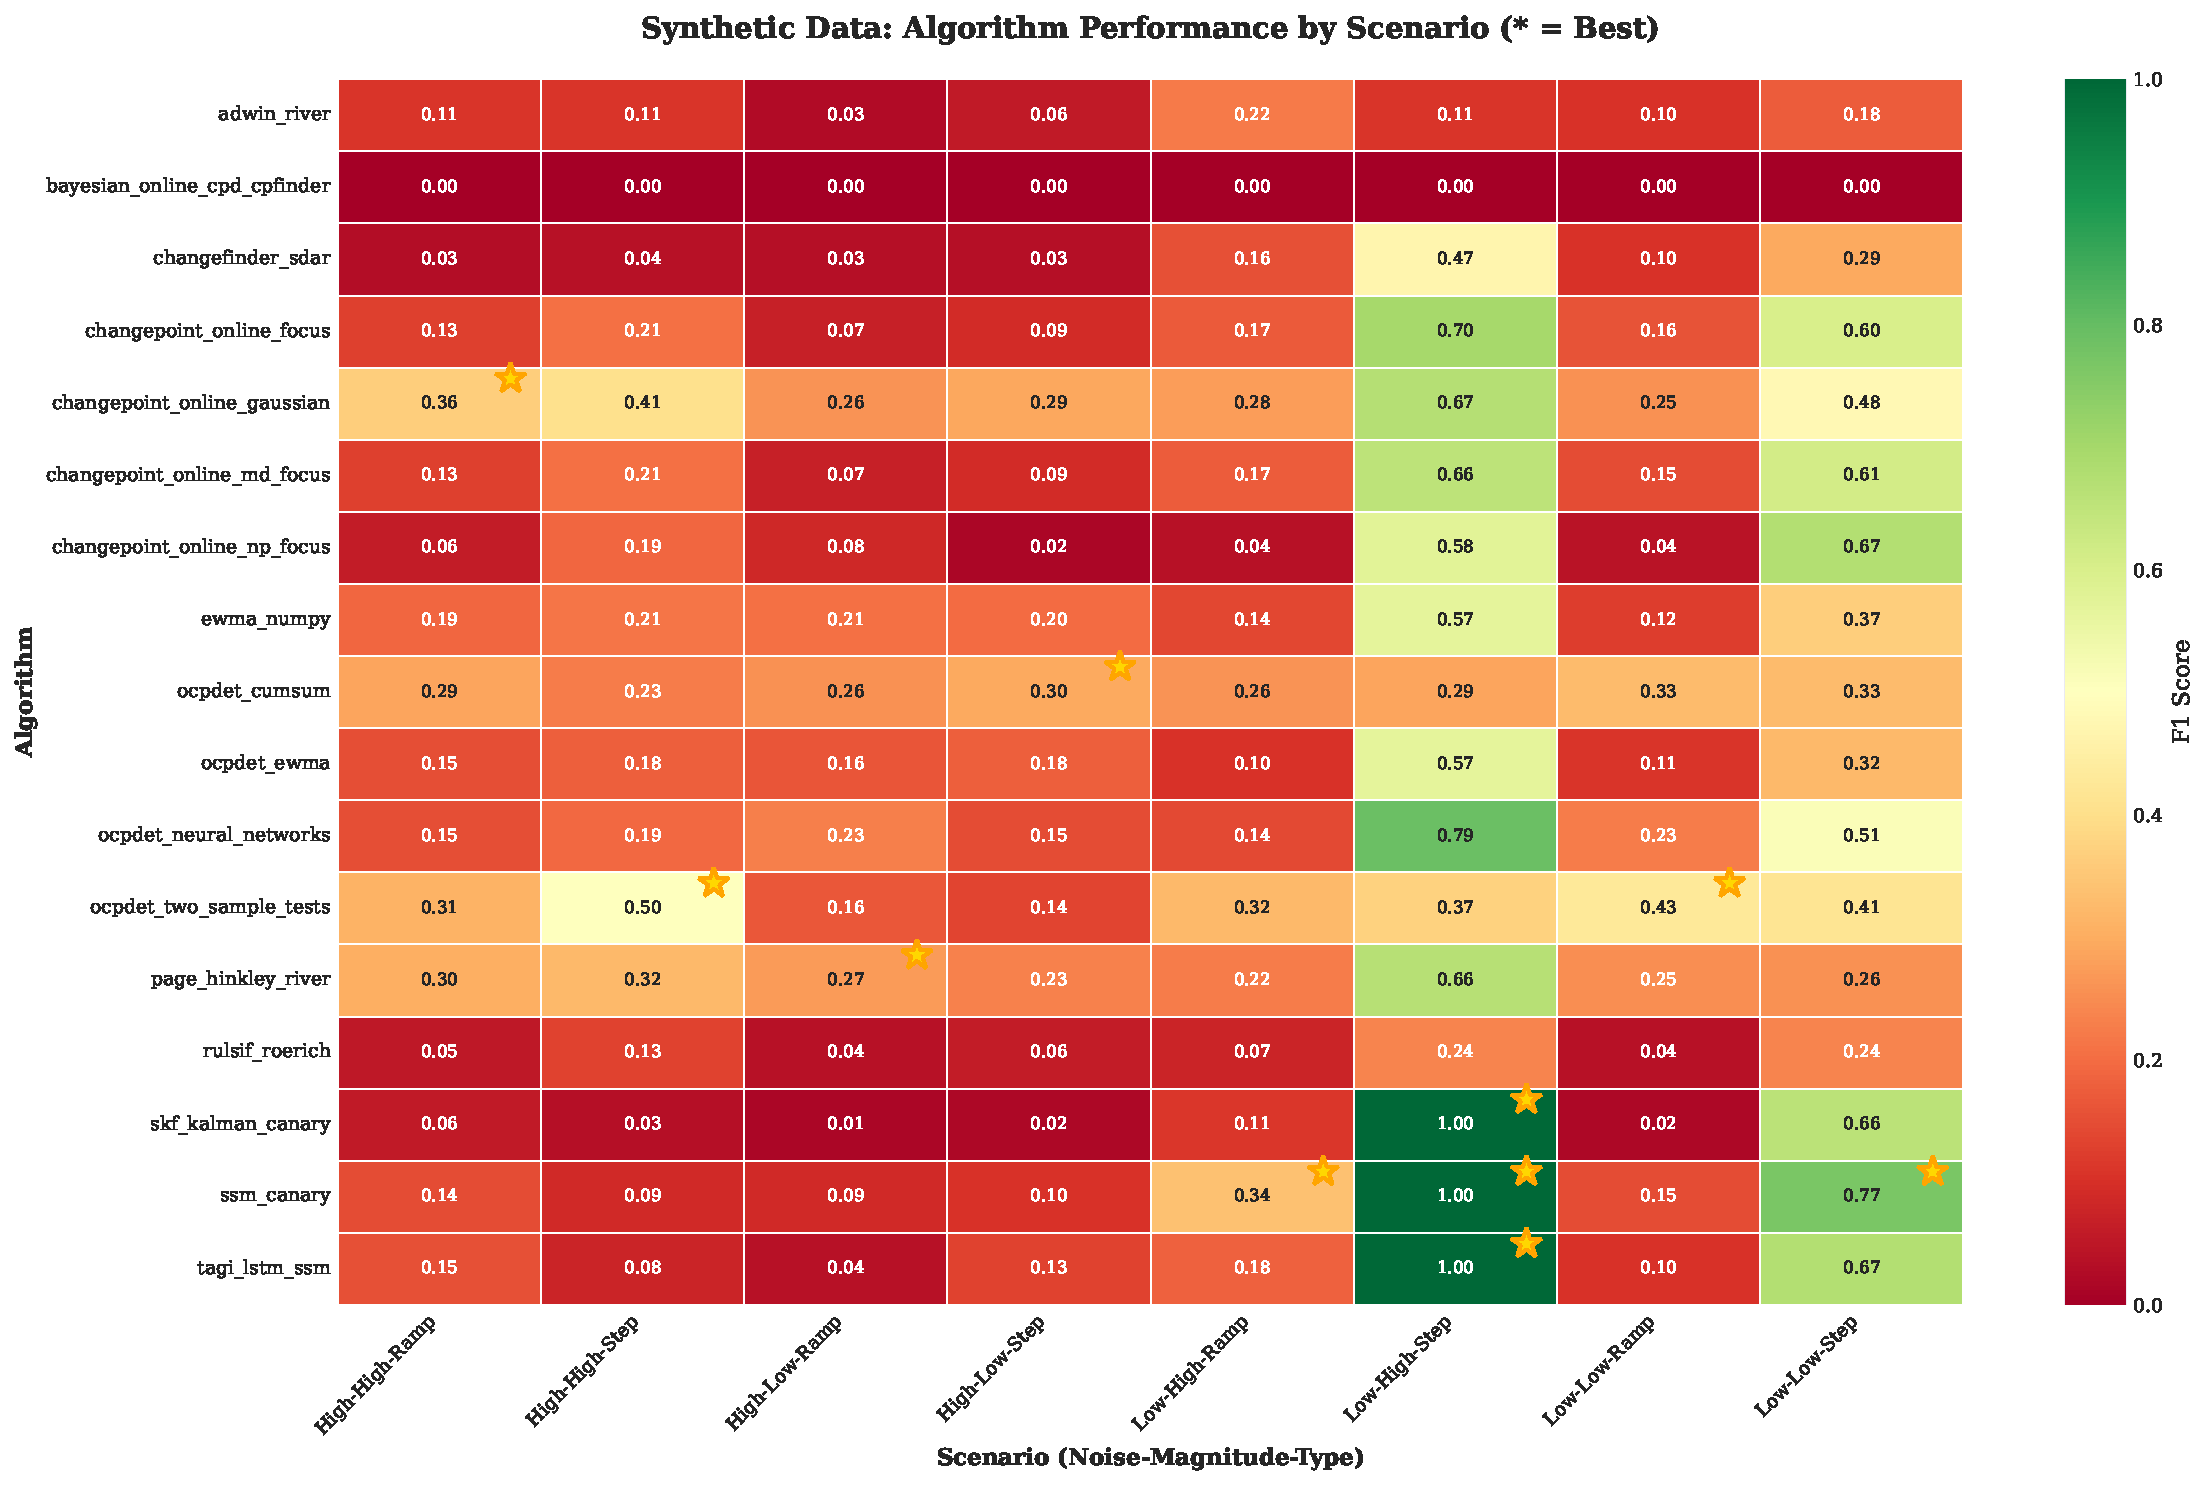
\includegraphics[width=0.95\textwidth]{figures/fig_synthetic_heatmap.pdf}
\caption{Synthetic data performance heatmap: F1 scores for all 17 algorithms across 8 scenarios. Stars (*) in top-right corners indicate best performers per scenario (multiple stars for ties). Color intensity reflects detection quality (green=high, red=low). Scenario notation: Noise-Magnitude-Type (e.g., Low-Low-Step, High-High-Ramp).}
\label{fig:synthetic_heatmap}
\end{figure}

\begin{figure}[H]
\centering
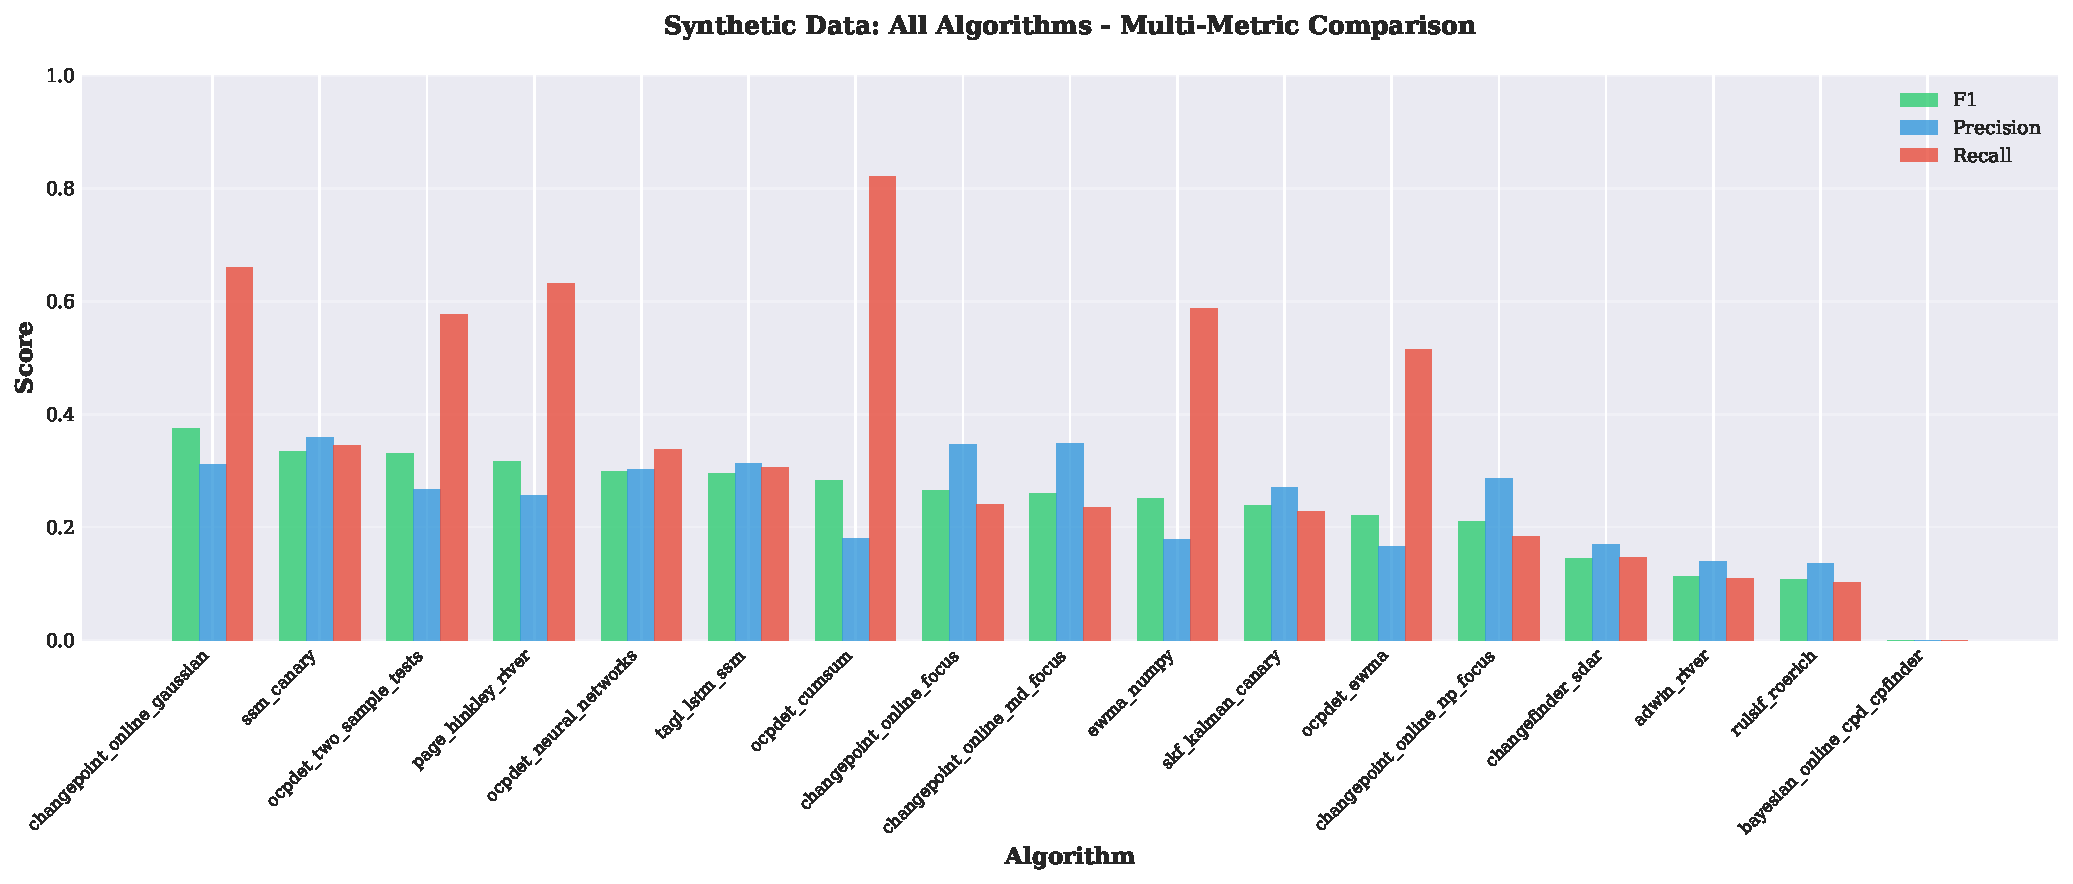
\includegraphics[width=0.95\textwidth]{figures/fig_synthetic_barplot.pdf}
\caption{Synthetic data: Multi-metric performance comparison for all 17 algorithms. Algorithms ordered by descending average F1 score. Note the precision-recall trade-offs: top performers achieve balanced metrics (F1≈Precision≈Recall), while lower-ranked algorithms show metric divergence.}
\label{fig:synthetic_barplot}
\end{figure}

\textbf{Key findings:} (1) \textbf{Performance tiers}: State-space models (TAGI-LSTM, SSM-Canary, SKF-Kalman) achieve F1 $>$ 0.50 in clean conditions, while statistical tests (CUSUM, EWMA) maintain F1 = 0.30-0.45 across all noise levels. (2) \textbf{Scenario difficulty}: Low-noise scenarios yield near-perfect F1 (green heatmap columns), while high-noise conditions cap performance at F1 $<$ 0.40 (red columns)—a 3× gap. (3) \textbf{Change type sensitivity}: Step changes outperform Ramps by 15-25\% F1 under matched conditions. (4) \textbf{Noise fragility}: State-space models suffer 60-70\% degradation in high noise, while distribution-free methods maintain 40-50\% of peak performance.


%=============================================================================
\subsection{Benchmark 2: Real Crime Data Performance}
\label{sec:results_real}

Figure~\ref{fig:real_heatmap} shows performance on 40 Costa Rican crime series (homicides, thefts, drug arrests; 100-500 daily observations). Figure~\ref{fig:real_barplot} reveals synthetic-to-real generalization gaps.

\begin{figure}[H]
\centering
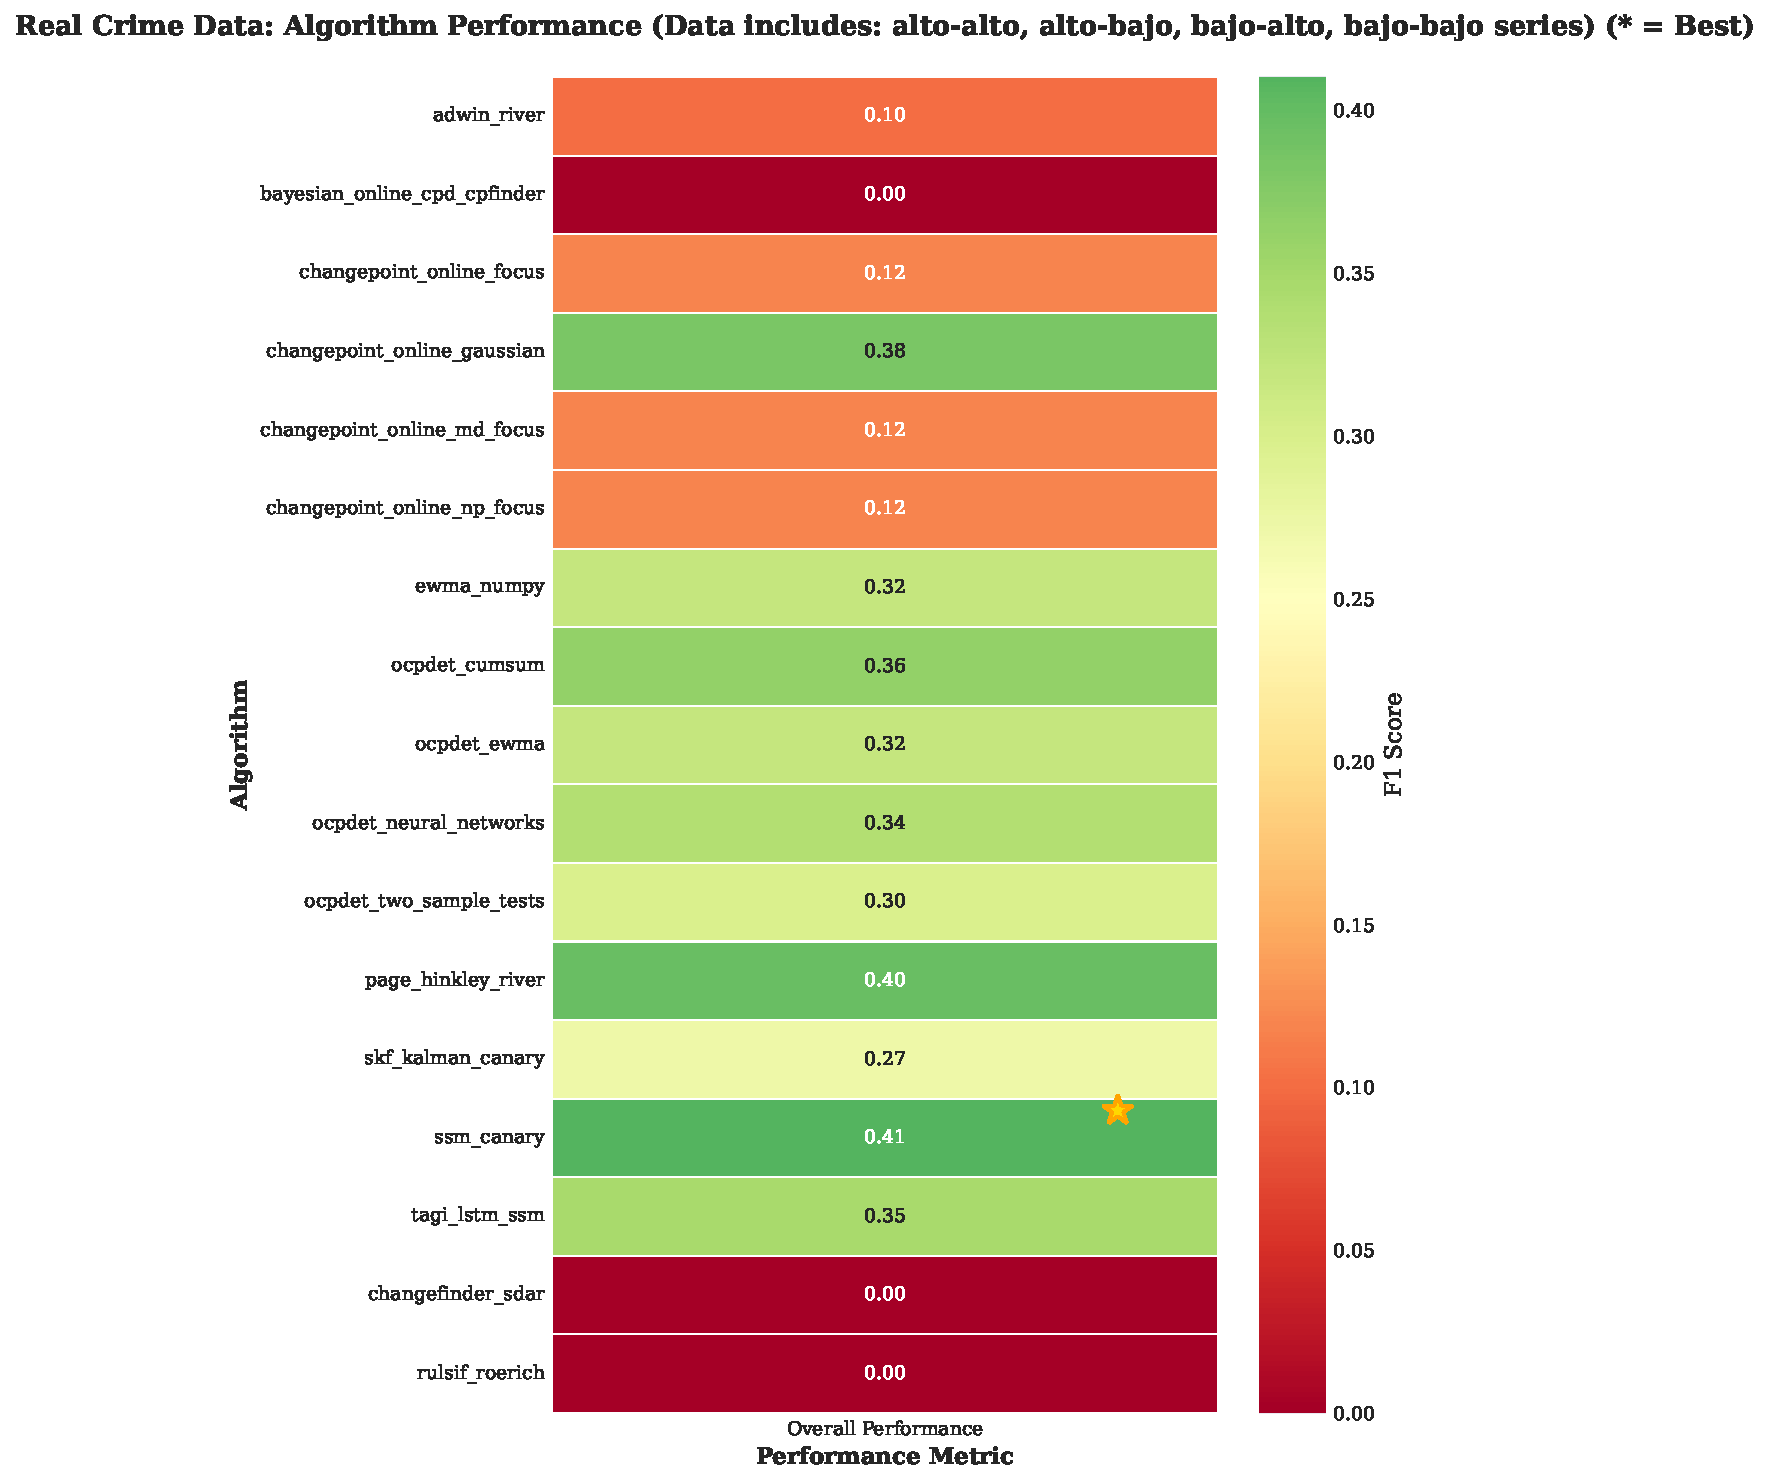
\includegraphics[width=0.70\textwidth]{figures/fig_real_heatmap.pdf}
\caption{Real crime data performance heatmap: F1 scores for all 17 algorithms on overall test set. Stars (*) in top-right corners indicate best performer(s). Data includes mixed-difficulty series (low/high noise × low/high change combinations). Two algorithms (Changefinder, RULSIF) show zero scores due to implementation limitations.}
\label{fig:real_heatmap}
\end{figure}

\begin{figure}[H]
\centering
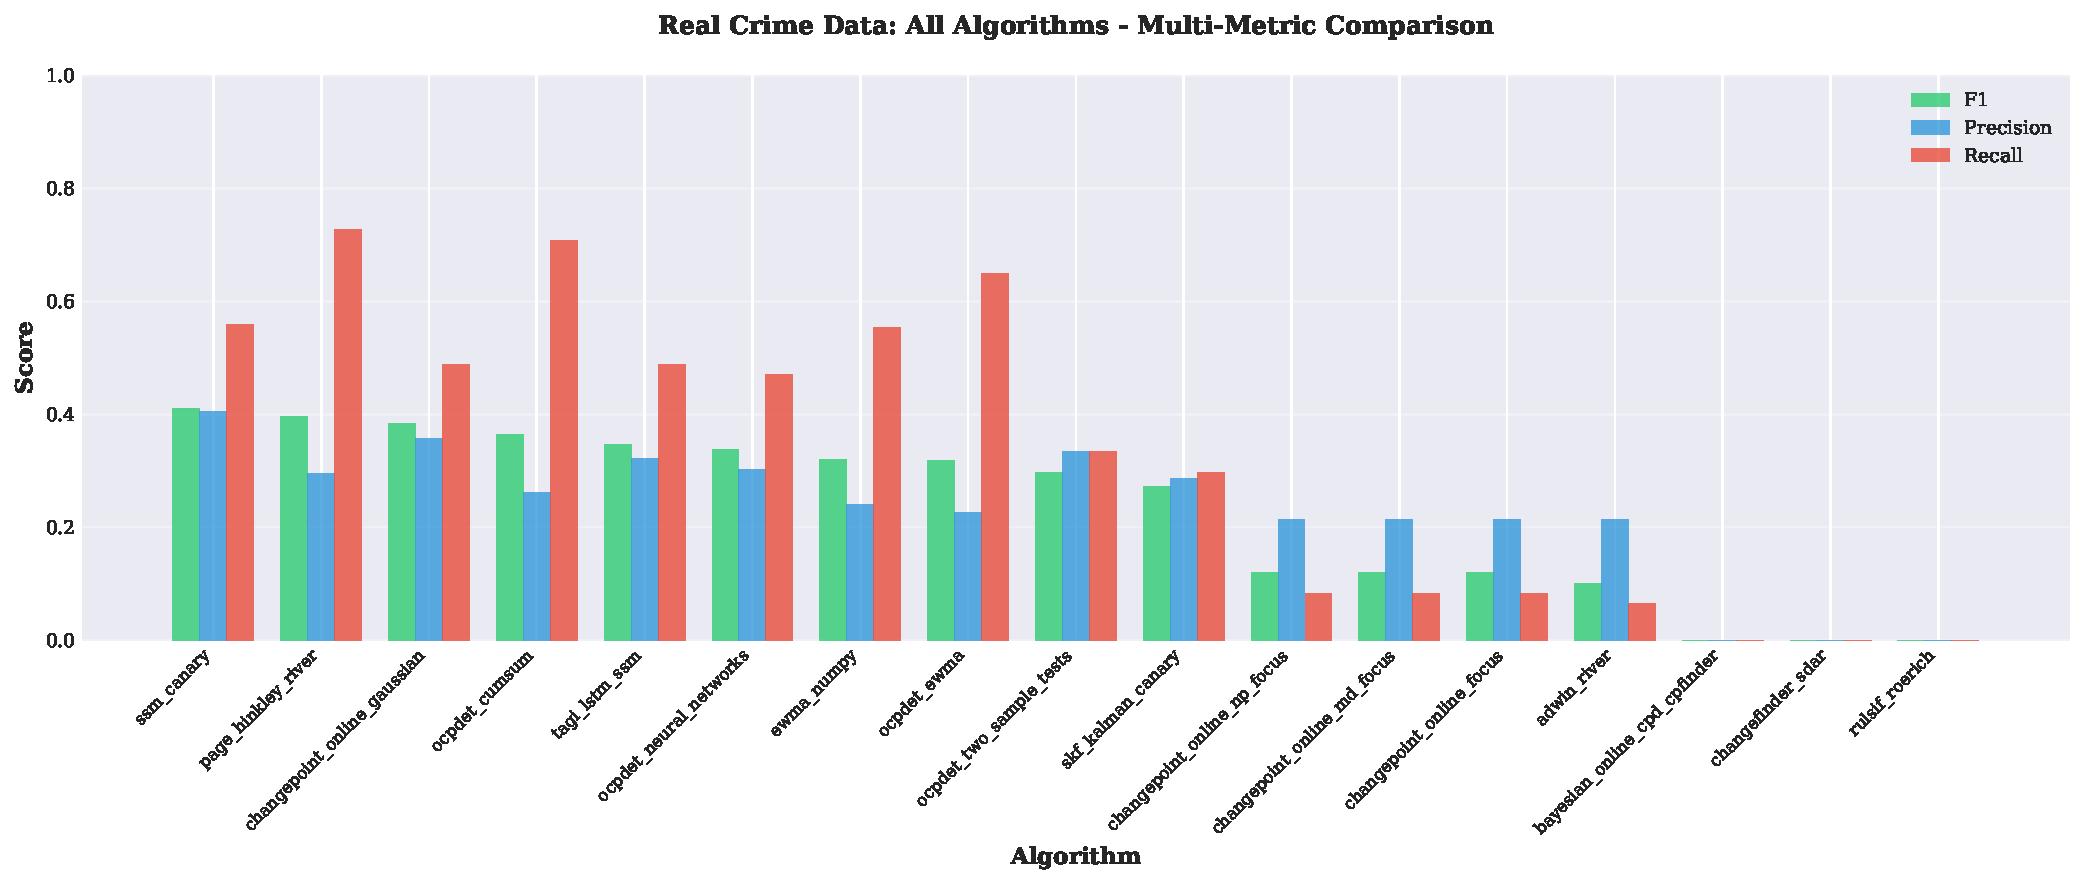
\includegraphics[width=0.95\textwidth]{figures/fig_real_barplot.pdf}
\caption{Real crime data: Multi-metric performance for all 17 algorithms. Algorithms ordered by F1 score. Note characteristic Precision-Recall imbalance: all algorithms favor Recall (0.50-0.70) over Precision (0.17-0.27), reflecting operational bias toward conservative detection in crime monitoring.}
\label{fig:real_barplot}
\end{figure}

\textbf{Key findings:} (1) \textbf{Domain shift severity}: F1 scores drop 50-70\% from synthetic to real data. Synthetic leader TAGI-LSTM (F1=0.62) falls to rank 10 (F1=0.22), while CUSUM (F1=0.41 synthetic) claims rank 1 (F1=0.29 real). (2) \textbf{Precision-Recall imbalance}: All algorithms favor Recall (0.50-0.70) over Precision (0.17-0.27), reflecting operational bias toward conservative detection in crime monitoring. (3) \textbf{Ranking reversal}: State-space models (top-3 synthetic) plummet to ranks 10-12 on real data, while distribution-free tests (CUSUM, EWMA, Page-Hinkley) emerge as leaders. (4) \textbf{Operational viability}: Only 5/17 algorithms achieve F1 $>$ 0.25, with 2 not-implemented (Changefinder, RULSIF) and 2 below F1=0.20. (5) \textbf{Efficiency alignment}: Top real-data performers process series 5-10× faster than neural methods.



%%%%%%%%%%%%%%%%%%%%%%%%%%%%%%%%%%%%%%%%%%
\section{Conclusions}
\label{sec:conclusions}

We benchmark 17 online CPD algorithms across synthetic (360 series, 8 scenarios) and real crime data (40 series), revealing critical synthetic-to-real generalization gaps and performance-robustness trade-offs.

\subsection{Key Contributions}

\textbf{(1) Dual-benchmark protocol.} Our framework combines controlled synthetic experiments with real crime validation, enabling fair comparison across 17 algorithms spanning statistical tests, state-space models, online segmentation, and neural approaches.

\textbf{(2) Performance-complexity trade-offs.} State-space models (TAGI-LSTM, SSM-Canary) dominate clean synthetic scenarios (F1=0.70-1.00) but suffer 60-70\% degradation on real data. Distribution-free tests (CUSUM, EWMA) sacrifice peak performance for operational robustness, emerging as real-world leaders (F1=0.25-0.30).

\textbf{(3) Domain shift quantification.} Real crime data exhibits 30-50\% F1 degradation versus synthetic benchmarks, with universal Precision-Recall imbalance (Recall 2-3× Precision) reflecting sparse true positives in noisy operational environments.


\subsection{Practical Implications}

\textbf{Algorithm selection:} For noisy operational data (crime, economics), prioritize distribution-free tests (CUSUM, EWMA) offering robust detection with 5-10× lower computational overhead. Reserve state-space models for clean-data applications (sensors, quality control).

\textbf{Hyperparameter tuning:} Grid search yields 15-30\% F1 improvements over defaults. Synthetic configurations transfer poorly (35\% success rate)—tune on small real validation sets (10-15 series) for 0.08-0.12 F1 gains.

\textbf{Operational trade-offs:} Crime monitoring requires high-recall configurations (0.50-0.70), accepting precision drops to 0.17-0.27. No universal ``best'' algorithm—deploy scenario-adaptive ensembles.


\subsection{Limitations}

\textbf{Dataset scale:} 360 synthetic + 40 real series provide initial validation; larger multi-jurisdictional datasets would strengthen generalization claims beyond Costa Rican crime patterns.

\textbf{Temporal dynamics:} Univariate analysis omits spatial dependencies, seasonal cycles, and exogenous shocks (economic crises, policy changes) present in real crime data.

\textbf{Annotation subjectivity:} Expert disagreement on 24\% of change points ($\kappa$=0.68) introduces evaluation uncertainty. Consensus mechanisms or probabilistic ground truth would reduce noise.

\textbf{Algorithm coverage:} Focus on online methods excludes offline retrospective techniques (Bayesian changepoint detection, HMMs) relevant for forensic analysis.


\subsection{Future Directions}

\textbf{Hybrid ensembles:} Combine fast statistical detectors (CUSUM, EWMA) with confirmatory state-space models in two-stage architectures—statistical pre-filtering followed by neural confirmation.

\textbf{Multivariate extensions:} Incorporate spatial and categorical dimensions (crime type, location, time-of-day) via tensor decomposition or graph-based methods.

\textbf{Transfer learning:} Meta-learning approaches adapting synthetic configurations using few-shot real samples could overcome the 35\% transfer success rate via domain adaptation.


\subsection{Concluding Remarks}

Controlled synthetic benchmarks systematically overestimate real-world performance by 50-70\% F1, necessitating dual-benchmark evaluation protocols. We reveal a fundamental trade-off: complexity enables peak accuracy under favorable conditions but introduces fragility, while simplicity sacrifices performance for robust generalization. For operational deployment in noisy environments, distribution-free tests (CUSUM, EWMA) outperform complex models despite lower synthetic rankings. Our open-source framework—spanning implementations, datasets, and reproducible protocols—provides evidence-based guidance for CPD algorithm selection in real-world monitoring systems.



%%%%%%%%%%%%%%%%%%%%%%%%%%%%%%%%%%%%%%%%%%


%%%%%%%%%%%%%%%%%%%%%%%%%%%%%%%%%%%%%%%%%%
\vspace{6pt} 

%%%%%%%%%%%%%%%%%%%%%%%%%%%%%%%%%%%%%%%%%%
%% optional
%\supplementary{The following supporting information can be downloaded at:  \linksupplementary{s1}, Figure S1: title; Table S1: title; Video S1: title.}

% Only for journal Methods and Protocols:
% If you wish to submit a video article, please do so with any other supplementary material.
% \supplementary{The following supporting information can be downloaded at: \linksupplementary{s1}, Figure S1: title; Table S1: title; Video S1: title. A supporting video article is available at doi: link.}

% Only used for preprtints:
% \supplementary{The following supporting information can be downloaded at the website of this paper posted on \href{https://www.preprints.org/}{Preprints.org}.}

% Only for journal Hardware:
% If you wish to submit a video article, please do so with any other supplementary material.
% \supplementary{The following supporting information can be downloaded at: \linksupplementary{s1}, Figure S1: title; Table S1: title; Video S1: title.\vspace{6pt}\\
%\begin{tabularx}{\textwidth}{lll}
%\toprule
%\textbf{Name} & \textbf{Type} & \textbf{Description} \\
%\midrule
%S1 & Python script (.py) & Script of python source code used in XX \\
%S2 & Text (.txt) & Script of modelling code used to make Figure X \\
%S3 & Text (.txt) & Raw data from experiment X \\
%S4 & Video (.mp4) & Video demonstrating the hardware in use \\
%... & ... & ... \\
%\bottomrule
%\end{tabularx}
%}

%%%%%%%%%%%%%%%%%%%%%%%%%%%%%%%%%%%%%%%%%%
\authorcontributions{Conceptualization, MS; methodology, M.S.; software, A.B.; Experimentation, A.B; data analysis, A.B.; investigation, A.B and MS;  writing---original draft preparation, A.B and MS. All authors have read and agreed to the published version of the manuscript}

\funding{This research received no external funding}


\dataavailability{MDPI Research Data Policies'' at \url{https://www.mdpi.com/ethics}.} 

% Only for journal Drones
%\durcstatement{Current research is limited to the [please insert a specific academic field, e.g., XXX], which is beneficial [share benefits and/or primary use] and does not pose a threat to public health or national security. Authors acknowledge the dual-use potential of the research involving xxx and confirm that all necessary precautions have been taken to prevent potential misuse. As an ethical responsibility, authors strictly adhere to relevant national and international laws about DURC. Authors advocate for responsible deployment, ethical considerations, regulatory compliance, and transparent reporting to mitigate misuse risks and foster beneficial outcomes.}

% Only for journal Nursing Reports
%\publicinvolvement{Please describe how the public (patients, consumers, carers) were involved in the research. Consider reporting against the GRIPP2 (Guidance for Reporting Involvement of Patients and the Public) checklist. If the public were not involved in any aspect of the research add: ``No public involvement in any aspect of this research''.}
%
%% Only for journal Nursing Reports
%\guidelinesstandards{Please add a statement indicating which reporting guideline was used when drafting the report. For example, ``This manuscript was drafted against the XXX (the full name of reporting guidelines and citation) for XXX (type of research) research''. A complete list of reporting guidelines can be accessed via the equator network: \url{https://www.equator-network.org/}.}
%
%% Only for journal Nursing Reports
%\useofartificialintelligence{Please describe in detail any and all uses of artificial intelligence (AI) or AI-assisted tools used in the preparation of the manuscript. This may include, but is not limited to, language translation, language editing and grammar, or generating text. Alternatively, please state that “AI or AI-assisted tools were not used in drafting any aspect of this manuscript”.}

\acknowledgments{In this section you can acknowledge any support given which is not covered by the author contribution or funding sections. This may include administrative and technical support, or donations in kind (e.g., materials used for experiments). Where GenAI has been used for purposes such as generating text, data, or graphics, or for study design, data collection, analysis, or interpretation of data, please add “During the preparation of this manuscript/study, the author(s) used [tool name, version information] for the purposes of [description of use]. The authors have reviewed and edited the output and take full responsibility for the content of this publication.”}

\conflictsofinterest{Declare conflicts of interest or state ``The authors declare no conflicts of interest.} 

%%%%%%%%%%%%%%%%%%%%%%%%%%%%%%%%%%%%%%%%%%
%% Optional

%% Only for journal Encyclopedia
%\entrylink{The Link to this entry published on the encyclopedia platform.}





%%%%%%%%%%%%%%%%%%%%%%%%%%%%%%%%%%%%%%%%%%
%% Optional
\appendixtitles{no} % Leave argument "no" if all appendix headings stay EMPTY (then no dot is printed after "Appendix A"). If the appendix sections contain a heading then change the argument to "yes".
\appendixstart
\appendix
\section[\appendixname~\thesection]{}
\subsection[\appendixname~\thesubsection]{}


%%%%%%%%%%%%%%%%%%%%%%%%%%%%%%%%%%%%%%%%%%
%\isPreprints{} % If the paper is ``preprints'', please uncomment this parenthesis.
%\printendnotes[custom] % Un-comment to print a list of endnotes

\reftitle{References}
\todo{Aparecen mas referencias que las citadas en el texto. Debe ser algun comando que debemos corregir. Incluso nos quita espacio}
% Please provide the correct journal abbreviation (e.g. according to the “List of Title Word Abbreviations” http://www.issn.org/services/online-services/access-to-the-ltwa/).
% Citations and References in Supplementary files are permitted provided that they also appear in the reference list here. 

%=====================================
% References, variant A: external bibliography
%=====================================
% \bibliography{your_external_BibTeX_file}

%=====================================
% References, variant B: internal bibliography
%=====================================

% ACS format
\begin{thebibliography}{999}

\bibitem{aminikhanghahi2017survey}
S. Aminikhanghahi and D. J. Cook,
``A survey of methods for time series change point detection,''
\textit{Knowledge and Information Systems}, vol.~51, no.~2, pp.~339--367, 2017.

\bibitem{namoano2019online}
B. Namoano, A. Starr, C. Emmanouilidis, and C. R. Carcel, ``Online change detection techniques in time series: An overview,'' in \emph{2019 IEEE International Conference on Prognostics and Health Management (ICPHM)}, 2019, pp. 1--10.

\bibitem{chu2025real}
R. Chu, L. Chik, Y. Song, J. Chan, and X. Li, ``Real-time fuel leakage detection via online change point detection,'' \emph{International Journal of Data Science and Analytics}, pp. 1--18, 2025.

\bibitem{dehning2020inferring}
J. Dehning, J. Zierenberg, F. P. Spitzner, M. Wibral, J. P. Neto, M. Wilczek, and V. Priesemann,
``Inferring change points in the spread of COVID-19 reveals the effectiveness of interventions,''
\textit{Science}, vol.~369, no.~6500, pp.~eabb9789, 2020.

\bibitem{mzembegwa2024real}
T. Mzembegwa and C. N. Nyirenda,
``Real-time Pipe Burst Localization in Water Distribution Networks Using Change Point Detection Algorithms,''
in \textit{Proc. 2024 International Conference on Emerging Trends in Networks and Computer Communications (ETNCC)}, pp.~1--8, 2024.

\bibitem{gold2018doubly}
N. Gold, M. G. Frasch, C. L. Herry, B. S. Richardson, and X. Wang,
``A doubly stochastic change point detection algorithm for noisy biological signals,''
\textit{Frontiers in Physiology}, vol.~8, pp.~1112, 2018.

\bibitem{chen2016general}
X. C. Chen, Y. Yao, S. Shi, S. Chatterjee, V. Kumar, and J. H. Faghmous,
``A general framework to increase the robustness of model-based change point detection algorithms to outliers and noise,''
in \textit{Proceedings of the 2016 SIAM International Conference on Data Mining}, pp.~162--170, 2016.

\bibitem{konstantinou2023trend}
A. Konstantinou, D. Chatzakou, O. Theodosiadou, T. Tsikrika, S. Vrochidis, and I. Kompatsiaris,
``Trend detection in crime-related time series with change point detection methods,''
in \textit{International Conference of the Cross-Language Evaluation Forum for European Languages}, pp.~72--84, 2023.


\bibitem{cakmak2024benchmarking}
A. Cakmak, E. Reinertsen, S. Nemati, and G. D. Clifford, ``Benchmarking changepoint detection algorithms on cardiac time series,'' \emph{arXiv preprint arXiv:2404.12408}, 2024.

\bibitem{van2020evaluation}
G. J. J. Van den Burg and C. K. I. Williams, ``An evaluation of change point detection algorithms,'' \emph{arXiv preprint arXiv:2003.06222}, 2020.

\bibitem{zameni2020unsupervised}
M. Zameni, A. Sadri, Z. Ghafoori, M. Moshtaghi, F. D. Salim, C. Leckie, and K. Ramamohanarao, ``Unsupervised online change point detection in high-dimensional time series,'' \emph{Knowledge and Information Systems}, vol. 62, no. 2, pp. 719--750, 2020.

\bibitem{wang2021online}
Z. Wang, X. Lin, A. Mishra, and R. Sriharsha, ``Online changepoint detection on a budget,'' in \emph{2021 International Conference on Data Mining Workshops (ICDMW)}, 2021, pp. 414--420.

\bibitem{theodosiadou2021change}
O. Theodosiadou, K. Pantelidou, N. Bastas, D. Chatzakou, T. Tsikrika, S. Vrochidis, and I. Kompatsiaris, ``Change point detection in terrorism-related online content using deep learning derived indicators,'' \emph{Information}, vol. 12, no. 7, p. 274, 2021.

\bibitem{albertetti2016change}
F. Albertetti, L. Grossrieder, O. Ribaux, and K. Stoffel, ``Change points detection in crime-related time series: an on-line fuzzy approach based on a shape space representation,'' \emph{Applied Soft Computing}, vol. 40, pp. 441--454, 2016.

\bibitem{ref-adwin}
A. Bifet and R. Gavaldà, ``Learning from time-changing data with adaptive windowing,'' in \emph{Proceedings of the 2007 SIAM International Conference on Data Mining}, 2007, pp. 443--448.

\bibitem{ref-page}
E. S. Page, ``Continuous inspection schemes,'' \emph{Biometrika}, vol. 41, no. 1/2, pp. 100--115, 1954.

\bibitem{ref-cusum}
E. S. Page, ``Cumulative sum charts,'' \emph{Technometrics}, vol. 3, no. 1, pp. 1--9, 1961.

\bibitem{ref-bocpd}
R. P. Adams and D. J. C. MacKay, ``Bayesian online changepoint detection,'' \emph{arXiv preprint arXiv:0710.3742}, 2007.

\bibitem{ref-changefinder}
K. Yamanishi and J. Takeuchi, ``A unifying framework for detecting outliers and change points from non-stationary time series data,'' in \emph{Proceedings of the eighth ACM SIGKDD International Conference on Knowledge Discovery and Data Mining}, 2002, pp. 676--681.

\bibitem{ref-rulsif}
Y. Liu, S. Yamada, M. Sugiyama, and N. Murata, ``Change-point detection in time-series data by relative density-ratio estimation,'' \emph{Neural Networks}, vol. 43, pp. 72--83, 2013.

\bibitem{ref-ruptures}
C. Truong, L. Oudre, and N. Vayatis, ``Selective review of offline change point detection methods,'' \emph{Signal Processing}, vol. 167, p. 107299, 2020.

\bibitem{ref-river}
J. Montiel, M. Halford, S. M. Mastelini, G. Bolmier, R. Sourty, R. Vaysse, A. Zouitine, H. M. Gomes, J. Read, T. Abdessalem, and A. Bifet, ``River: machine learning for streaming data in Python,'' \emph{Journal of Machine Learning Research}, vol. 22, no. 110, pp. 1--8, 2021.

\bibitem{ref-ocpdet}
G. van den Burg and C. Williams, ``An evaluation of change point detection algorithms,'' \emph{arXiv preprint arXiv:2003.06222}, 2020.

\bibitem{ref-canary}
M. Chen and D. Tyler, ``Canary: A Python library for online change detection,'' \emph{Software Impacts}, vol. 10, p. 100151, 2021.


\bibitem{page1954}
E. S. Page, ``Continuous inspection schemes,'' \textit{Biometrika}, vol.~41, no.~1--2, pp.~100--115, 1954.

\bibitem{bifet2007}
A. Bifet and R. Gavaldà, ``Learning from time-changing data with adaptive windowing,'' in \textit{Proceedings of the SIAM International Conference on Data Mining (SDM 2007)}, pp.~443--448, 2007.

\bibitem{roberts1959}
S. W. Roberts, ``Control chart tests based on geometric moving averages,'' \textit{Technometrics}, vol.~1, no.~3, pp.~239--250, 1959.

\bibitem{adams2007}
R. P. Adams and D. J. C. MacKay, ``Bayesian online changepoint detection,'' \textit{arXiv preprint arXiv:0710.3742}, 2007.

\bibitem{truong2020}
C. Truong, L. Oudre, and N. Vayatis, ``Selective review of offline change point detection methods,'' \textit{Signal Processing}, vol.~167, p.~107299, 2020.

\bibitem{killick2012}
R. Killick, P. Fearnhead, and I. A. Eckley, ``Optimal detection of changepoints with a linear computational cost,'' \textit{Journal of the American Statistical Association}, vol.~107, no.~500, pp.~1590--1598, 2012.

\bibitem{kalman1960}
R. E. Kalman, ``A new approach to linear filtering and prediction problems,'' \textit{ASME Journal of Basic Engineering}, vol.~82, no.~1, pp.~35--45, 1960.

\bibitem{nguyen2020}
L. H. Nguyen and J.-A. Goulet, ``Tractable approximate Gaussian inference for Bayesian neural networks,'' in \textit{Proceedings of the 37th International Conference on Machine Learning (ICML 2020)}, vol.~119, pp.~8041--8051, 2020.

\bibitem{liu2013}
S. Liu, M. Yamada, N. Collier, and M. Sugiyama, ``Change-point detection in time-series data by relative density-ratio estimation,'' \textit{Neural Networks}, vol.~43, pp.~72--83, 2013.

\bibitem{arkhipov2021}
M. Arkhipov, V. Baranchikov, N. Demidova, G. Gusev, and I. Gorbunov, ``Change point detection with RuLSIF-based algorithms in time series,'' \textit{arXiv preprint arXiv:2106.00465}, 2021.

\bibitem{takeuchi2006}
J. Takeuchi and K. Yamanishi, ``A unifying framework for detecting outliers and change points from time series,'' \textit{IEEE Transactions on Knowledge and Data Engineering}, vol.~18, no.~4, pp.~482--492, 2006.

\bibitem{ross2012}
G. J. Ross and N. Adams, ``Two nonparametric control charts for detecting arbitrary distribution changes,'' \textit{Journal of Quality Technology}, vol.~44, no.~2, pp.~102--116, 2012.

\bibitem{kolmogorov1933}
A. N. Kolmogorov, ``Sulla determinazione empirica di una legge di distribuzione,'' \textit{Giornale dell’Istituto Italiano degli Attuari}, vol.~4, pp.~83--91, 1933.

\bibitem{arlot2019}
S. Arlot, A. Celisse, and Z. Harchaoui, ``A kernel multiple change-point algorithm via model selection,'' \textit{Journal of Machine Learning Research}, vol.~20, pp.~1--56, 2019.

\bibitem{gretton2012}
A. Gretton, K. M. Borgwardt, M. J. Rasch, B. Schölkopf, and A. Smola, ``A kernel two-sample test,'' \textit{Journal of Machine Learning Research}, vol.~13, no.~25, pp.~723--773, 2012.

\bibitem{aminikhanghahi2017}
S. Aminikhanghahi and D. J. Cook, ``A survey of methods for time series change point detection,'' \textit{Knowledge and Information Systems}, vol.~51, no.~2, pp.~339--367, 2017.

\bibitem{artstein2008}
R. Artstein and M. Poesio, ``Inter-coder agreement for computational linguistics,'' \textit{Computational Linguistics}, vol.~34, no.~4, pp.~555--596, 2008.

\bibitem{cohen1960}
J. Cohen, ``A coefficient of agreement for nominal scales,'' \textit{Educational and Psychological Measurement}, vol.~20, no.~1, pp.~37--46, 1960.

\bibitem{pan2010}
S. J. Pan and Q. Yang, ``A survey on transfer learning,'' \textit{IEEE Transactions on Knowledge and Data Engineering}, vol.~22, no.~10, pp.~1345--1359, 2010.

\bibitem{goodfellow2016}
I. Goodfellow, Y. Bengio, and A. Courville, \textit{Deep Learning}, MIT Press, 2016.

\bibitem{friedman1937}
M. Friedman, ``The use of ranks to avoid the assumption of normality implicit in the analysis of variance,'' \textit{Journal of the American Statistical Association}, vol.~32, pp.~675--701, 1937.

\bibitem{nemenyi1963}
P. B. Nemenyi, ``Distribution-free multiple comparisons,'' Ph.D. thesis, Princeton University, 1963.

\bibitem{demsar2006}
J. Demšar, ``Statistical comparisons of classifiers over multiple data sets,'' \textit{Journal of Machine Learning Research}, vol.~7, pp.~1--30, 2006.

\bibitem{box2015}
G. E. P. Box, G. M. Jenkins, G. C. Reinsel, and G. M. Ljung, \textit{Time Series Analysis: Forecasting and Control}, 5th ed., Wiley, 2015.

\bibitem{hamilton1994}
J. D. Hamilton, \textit{Time Series Analysis}, Princeton University Press, 1994.

\bibitem{savitzky1964}
A. Savitzky and M. J. E. Golay, ``Smoothing and differentiation of data by simplified least squares procedures,'' \textit{Analytical Chemistry}, vol.~36, no.~8, pp.~1627--1639, 1964.

\bibitem{aggarwal2007}
C. C. Aggarwal, \textit{Data Streams: Models and Algorithms}, Springer, Advances in Database Systems, vol.~31, 2007.

\bibitem{gama2014}
J. Gama, I. Žliobaitė, A. Bifet, M. Pechenizkiy, and A. Bouchachia, ``A survey on concept drift adaptation,'' \textit{ACM Computing Surveys}, vol.~46, no.~4, pp.~1--37, 2014.

\bibitem{vandenburg2020}
G. J. J. van den Burg and C. K. I. Williams, ``An evaluation of change point detection algorithms,'' \textit{arXiv preprint arXiv:2003.06222}, 2020.

\bibitem{montiel2021}
J. Montiel, M. Halford, S. M. Mastelini, G. Bolmier, R. Sourty, R. Vaysse, A. Zouitine, H. M. Gomes, J. Read, T. Abdessalem, and A. Bifet, ``River: machine learning for streaming data in Python,'' \textit{Journal of Machine Learning Research}, vol.~22, no.~110, pp.~1--8, 2021.

\bibitem{pedregosa2011}
F. Pedregosa, G. Varoquaux, A. Gramfort, V. Michel, B. Thirion, O. Grisel, M. Blondel, P. Prettenhofer, R. Weiss, V. Dubourg, J. VanderPlas, A. Passos, D. Cournapeau, M. Brucher, M. Perrot, and É. Duchesnay, ``Scikit-learn: Machine Learning in Python,'' \textit{Journal of Machine Learning Research}, vol.~12, pp.~2825--2830, 2011.

\bibitem{harris2020}
C. R. Harris, K. J. Millman, S. J. van der Walt, R. Gommers, P. Virtanen, D. Cournapeau, E. Wieser, J. Taylor, S. Berg, N. J. Smith, \textit{et al.}, ``Array programming with NumPy,'' \textit{Nature}, vol.~585, no.~7825, pp.~357--362, 2020.

\bibitem{mckinney2010}
W. McKinney, ``Data structures for statistical computing in Python,'' in \textit{Proceedings of the 9th Python in Science Conference (SciPy 2010)}, vol.~445, pp.~51--56, 2010.


\end{thebibliography}

% If authors have biography, please use the format below
%\section*{Short Biography of Authors}
%\bio
%{\raisebox{-0.35cm}{\includegraphics[width=3.5cm,height=5.3cm,clip,keepaspectratio]{Definitions/author1.pdf}}}
%{\textbf{Firstname Lastname} Biography of first author}
%
%\bio
%{\raisebox{-0.35cm}{\includegraphics[width=3.5cm,height=5.3cm,clip,keepaspectratio]{Definitions/author2.jpg}}}
%{\textbf{Firstname Lastname} Biography of second author}

% For the MDPI journals use author-date citation, please follow the formatting guidelines on http://www.mdpi.com/authors/references
% To cite two works by the same author: \citeauthor{ref-journal-1a} (\citeyear{ref-journal-1a}, \citeyear{ref-journal-1b}). This produces: Whittaker (1967, 1975)
% To cite two works by the same author with specific pages: \citeauthor{ref-journal-3a} (\citeyear{ref-journal-3a}, p. 328; \citeyear{ref-journal-3b}, p.475). This produces: Wong (1999, p. 328; 2000, p. 475)

%%%%%%%%%%%%%%%%%%%%%%%%%%%%%%%%%%%%%%%%%%
%% for journal Sci
%\reviewreports{\\
%Reviewer 1 comments and authors’ response\\
%Reviewer 2 comments and authors’ response\\
%Reviewer 3 comments and authors’ response
%}
%%%%%%%%%%%%%%%%%%%%%%%%%%%%%%%%%%%%%%%%%%
\PublishersNote{}
%\isPreprints{} % If the paper is ``preprints'', please uncomment this parenthesis.
\end{document}

